\section{Linear System Identification}
\label{sec:sysid}

%% Overview of this section
Any finite-dimensional, Lipschitz continuous nonlinear dynamical system has an equivalent infinite-dimensional linear representation that acts on the space of all real-valued functions on the system's state \cite[Definition 3.3.1]{lasota2013chaos}.
This linear representation, which is called the Koopman operator, describes the flow of functions along trajectories of the system.
% The dual of the Koopman operator, the Perron-Frobenius operator, describes the dynamics of the system...
While it is not possible to numerically represent the infinite-dimensional Koopman operator, it is possible to construct its projection onto a finite-dimensional subspace using a matrix.
% Our goal is to construct models in this subspace in the form of a controlled linear dynamical system
% \begin{align}
%     \psi_{k+1} &= A \psi_{k} + B u_{k} \\
%     y_{k} &= C \psi_{k}
% \end{align}
% where $z$ is ... , $u$ is the input, and $y$ is the output of the system.
This section shows that for a given choice of basis functions, a \emph{lifted} linear dynamical system model can be extracted directly from the matrix approximation of the Koopman operator.
% As desired, system representations of this form lend themselves to linear control methods.
The remainder of this sections outlines the approach for constructing the Koopman operator approximation and the linear system representation from data.
Section \ref{sec:mpc} illustrates how this model can be incorporated into a model predictive control algorithm.

%% Overview of the Koopman operator and how it represents dynamical systems
\subsection{Koopman Representation of a Dynamical System}

%% System representation in state space
Consider a dynamical system
\begin{align}
    \dot{x}(t) &= F (x(t))
    \label{eq:nlsys}
\end{align}
where $x(t) \in \Real^n$ is the state of the system at time $t \geq 0$, and ${F}$ is a continuously differentiable function.
Denote by $\phi(t,x_0)$ the solution to \eqref{eq:nlsys} at time $t$ when beginning with the initial condition $x_0$ at time $0$.
For simplicity, we denote this map, which is referred to as the \emph{flow map}, by $\phi_t (x_0)$ instead of $\phi (t, x_0)$.

%% System representation in the space of observables
The system can be lifted to an infinite dimensional function space $\mathcal{F}$ composed of all square integrable real-valued functions with compact domain $X \subset \Real^n$.
Elements of $\mathcal{F}$ are called \emph{observables}.
In $\mathcal{F}$, the flow of the system is characterized by the set %semigroup 
of Koopman operators 
$U_t : \mathcal{F} \to \mathcal{F}$, for each $t \geq 0$,
which describes the evolution of the observables ${f \in \mathcal{F}}$ along the trajectories of the system according to the following definition:
\begin{align}
    U_t f = f \circ \phi_t      
    % && \forall f \in \F, t \geq 0
    \label{eq:koopman}
\end{align}
As desired, $U_t$ is a linear operator even if the system \eqref{eq:nlsys} is nonlinear, since for $f_1, f_2 \in \mathcal{F}$ and $\lambda_1, \lambda_2 \in \Real$
\begin{align}
    \begin{split}
    U_t (\lambda_1 f_1 + \lambda_2 f_2) &= \lambda_1 f_1 \circ \phi_t + \lambda_2 f_2 \circ \phi_t \\
    &= \lambda_1 U_t f_1 + \lambda_2 U_t f_2.
    \end{split}
\end{align}
Thus the Koopman operator provides a linear representation of the flow of a nonlinear system in the infinite-dimensional space of observables (see Fig. \ref{fig:overview}) \cite{budivsic2012applied}.
Contrast this representation with the one generated by the (nonlinear) flow map which for each $t \geq 0$ describes how the initial condition evolves according to the dynamics of the system.
In particular if one wants to understand the evolution of an initial condition $x_0$ at time $t$ according to \eqref{eq:nlsys}, then one could solve the nonlinear differential equation to generate the flow map. 
On the other hand, one could apply $U_t$ (a linear operator) to the indicator function centered at $x_0$ to generate an indicator function centered at the point where $x_0$ reaches at time $t$ while satisfying \eqref{eq:nlsys}. 
% \Ram{you need to say something more explicit here. While $\phi$ describes how an initial condition flows according to the ODE, the Koopman operator describes how a function evolves according to the ODE. Notice that one can go back and forth between the representations...}.


%% Koopman-based system identification (consult ICRA paper)
\subsection{Identification of Koopman Operator}
\label{sec:koopid}

Since the Koopman operator is an infinite-dimensional object, it cannot be represented by a finite-dimensional matrix. 
Therefore, we settle for the projection of the Koopman operator onto a finite-dimensional subspace.
Using a modified version of the Extended Dynamic Mode Decomposition (EDMD) algorithm \cite{williams2015data} originally presented in \cite{mauroy2016linear,mauroy2017koopman}, we identify a finite-dimensional approximation of the Koopman operator via linear regression applied to the observed data.

Define ${\bar{\mathcal{F}} \subset \mathcal{F}}$ to be the subspace of $\mathcal{F}$ spanned by ${N>n}$ linearly independent basis functions 
${ \{ \psi_i : \Real^n \to \Real \}_{i=1}^N}$.
We denote the image of $\psi_k$ as $ \mathcal{R}_k$ which is equal to $\{ w \in \Real | \exists x \in \Real^n \text{ such that } \psi_i(x) = w  \}$.
For convenience, we assume that the first $n$ basis functions are defined as
\begin{align}
    &\psi_i(x) = x_i
    \label{eq:xinpsi}
\end{align}
where $x_i$ denotes the $i^{\text{th}}$ coordinate of $x$.
Any observable $\bar{f} \in \bar{\mathcal{F}}$ can be expressed as a linear combination of elements of these basis functions
\begin{align}
    \bar{f} &= \theta_1 \psi_1 + \cdots + \theta_N \psi_N
    \label{eq:fexpanded}
\end{align}
where each $\theta_i \in \Real$.
For convenience in presentation, we introduce the vector of coefficients ${\theta = [ \theta_1 \,  \cdots \, \theta_N ]^\top}$ and the \emph{lifting function} ${\psi : \Real^n \to \Real^N}$ defined as:
\begin{align}
    \psi(x) &:= \begin{bmatrix} \psi_1 (x) & \cdots & \psi_N (x) \end{bmatrix}^\top.
    \label{eq:lift}
\end{align}
We denote the image of $\psi$ as $\mathcal{M} = \mathcal{R}_1 \times \cdots \times \mathcal{R}_N \subset \Real^N$.
By \eqref{eq:fexpanded} and \eqref{eq:lift}, $\bar{f}$ evaluated at a point $x$ in the state space is given by
% Note that $\bar{\theta}$ provides a vector representation for ${ \bar{f} \in \bar{\mathcal{F}} }$, and $\bar{f}$ evaluated at a point $x$ is given by
% Then, $\bar{f} \in \bar{\mathcal{F}}$ can be expressed concisely as
\begin{align}
    \bar{f}(x) &= \theta^\top \psi (x)
    \label{eq:fvec}
\end{align}
We therefore refer to $\psi(x)$ as the \emph{lifted state}, and $\theta$ as the \emph{vector representation} of $\bar{f}$.

Given this vector representation for observables, a linear operator $L : \bar{\mathcal{F}} \to \bar{\mathcal{F}}$ can be represented as an ${N \times N}$ matrix. 
We denote by $\bar{U}_t \in \Real^{N \times N}$ the approximation of the Koopman operator in $\bar{\mathcal{F}}$, which operates on observables via matrix multiplication:
\begin{align}
    \bar{U}_t \theta = \theta'
\end{align}
where $\theta , \theta'$ are each vector representations of observables in $\bar{\mathcal{F}}$.
%% Pulled straight from ICRA paper below this line
Our goal is to find a $\bar{U}_t$ that describes the action of the infinite dimensional Koopman operator $U_t$ as accurately as possible in the $L^2$-norm sense on the finite dimensional subspace $\bar{\mathcal{F}}$ of all observables.

To perfectly mimic the action of $U_t$ on an observable ${f \in \bar{\mathcal{F}} \subset \mathcal{F}}$, according to \eqref{eq:koopman} the following should be true for all $x \in \Real^n$
\begin{align}
    \bar{U}_t \bar{f}(x) &= \bar{f} \circ \phi_t (x) \\
    ( \bar{U}_t {\theta} )^\top {\psi}(x) &=
    {\theta}^\top {\psi} \circ \phi_t(x) \\
    \bar{U}_t^\top \psi(x) &= {\psi} \circ \phi_t(x),
    \label{eq:UbarEq}
\end{align}
where the second equation follows by substituting \eqref{eq:fexpanded} and the last equation follows by cancelling $\theta^\top$.
Since this is a linear equation, it follows that for a given ${x \in \Real^n}$, solving \eqref{eq:UbarEq} for $\bar{U}_t$ yields the best approximation of $U_t$ on $\bar{\mathcal{F}}$ in the $L^2$-norm sense \cite{penrose1956best}:
\begin{align}
    \bar{U}_t = \left( {\psi}(x)^\top \right)^\dagger {\psi}( \phi_t(x) )^\top
    \label{eq:Uapprox}
\end{align}
where superscript $\dagger$ denotes the least-squares pseudoinverse.

%% How this is done on our system
To approximate the Koopman operator from a set of experimental data, we take $K$ discrete state measurements in the form of so-called ``snapshot pairs'' $(a[k] , b[k])$ for each $k \in \{1,\ldots,K\}$ where
% with sampling period $T_s$. We separate the data into a set of $K$ so-called ``snapshot pairs'' of the form ${ \{ a_k , b_k \} \in \Real^{n \times 2} }$ where
\begin{align}
    a[k] &= x[k] \\
    b[k] &= \phi_{T_s} (x[k]) + \sigma[k],
    \label{eq:ab}
\end{align}
$\sigma_k$ denotes measurement noise, $T_s$ is the sampling period which is assumed to be identical for all snapshot pairs, and $x[k]$ denotes the measured state corresponding to the $k^\text{th}$ measurement.
\Ram{is this where we mention that these measurements do not have to correspond to the state of the system but rather the things we can observe?}
Note that consecutive snapshot pairs do not have to be generated by consecutive state measurements. 
% For our basis of $\bar{\mathcal{F}}$, we choose the basis of monomials of $x$ with total degree less than or equal to $w$, which implies ${N=(n+m+w)!/\left((n+m)!w!\right)}$ \cite[Section III]{mauroy2016linear}. 
We then lift all of the snapshot pairs according to \eqref{eq:lift} and compile them into the following ${K \times N}$ matrices:
\begin{align}
    &\Psi_a := \begin{bmatrix} {\psi}(a[1])^\top \\ \vdots \\  {\psi}(a[K])^\top \end{bmatrix}
    &&\Psi_b := \begin{bmatrix} {\psi}(b[1])^\top \\ \vdots \\  {\psi}(b[K])^\top \end{bmatrix}
    \label{eq:Psi}
\end{align}
$\bar{U}_{T_s}$ is chosen so that it yields the least-squares best fit to all of the observed data, which, following from \eqref{eq:Uapprox}, is given by 
\begin{align}
    \bar{U}_{T_s} &:= \Psi_a^\dagger \Psi_b.
\end{align}

%% Incorporating Delays
Sometimes a more accurate model can be attained by incorporating delays into the set of snapshot pairs. 
To incorporate these delays, we define the snapshot pairs as
\begin{align}
    a[k] &= \begin{bmatrix} x[k]^\top & x[k-1]^\top & \ldots & x[k-d]^\top \end{bmatrix}^\top \label{eq:snapd1} \\
    b[k] &= \begin{bmatrix} \left( \phi_{T_s} (x[k]) + \sigma_k \right)^\top & x[k]^\top & \ldots & x[k-d+1]^\top \end{bmatrix}^\top \label{eq:snapd2}
\end{align}
where $d$ is the number of delays.
We then modify the domain of the lifting function such that $\psi : \Real^{n+nd} \to \Real^{N}$ to accommodate the larger dimension of the snapshot pairs.
Once these snapshot pairs have been assembled, the model identification procedure is identical to the case without delays.
% without input delays or $\Real^{n+nd} \times \Real^{md}$ with input delays.

%% Koopman representation of controlled dynamical system
\subsection{Building Linear System from Koopman Operator}
%Brent: Building a Linear Model from the Koopman Operator
% I don't get the lack of articles in your section heading. 

For dynamical systems with inputs, we are interested in using the Koopman operator to construct discrete linear models of the following form
\begin{equation}
\begin{aligned}
    z[j+1] &= A z[j] + B u[j] \\
    x[j] &= C z[j]
    \label{eq:linSys}
\end{aligned}
\end{equation}
 for each $j \in \mathbb{N}$ where $x[0]$ is the initial condition in state space, $z[0] = \psi(x[0])$, and $u[j] \in \Real^m$ is the input at the $j^{\text{th}}$ step.
Specifically, we desire a representation in which (non-lifted) inputs appear \emph{linearly}, because models of this form are amenable to real-time, convex optimization techniques for feedback control design as we describe in Section \ref{sec:mpc}.

We construct a model of this form by first applying the system identification method of Section \ref{sec:koopid} to the modified snapshot pairs
% \begin{align}
%     \alpha_k &= \begin{bmatrix} \psi(a_k)^\top & u_k^\top \end{bmatrix} \\
%     \beta_k &= \begin{bmatrix} \psi(b_k)^\top & u_k^\top \end{bmatrix} 
% \end{align}
\begin{align}
    &\alpha[k] = \begin{bmatrix} \psi(a[k]) \\ u[k] \end{bmatrix} 
    &&\beta[k] = \begin{bmatrix} \psi(b[k]) \\ u[k] \end{bmatrix}.
    \label{eq:alpha}
\end{align}
for each $k \in \{1,\ldots,K\}$. 
The input $u[k]$ in snapshot $k$ is not lifted to ensure that it appears linearly in the resulting model.
With these pairs, we define the following ${K \times (N + m)}$ matrices:
\begin{align}
    &\Gamma_\alpha = \begin{bmatrix} \alpha[1]^\top \\ \vdots \\  \alpha[K]^\top \end{bmatrix}
    &&\Gamma_\beta = \begin{bmatrix} \beta[1]^\top \\ \vdots \\  \beta[K]^\top \end{bmatrix}
    \label{eq:Gamma}
\end{align}
and solve for the corresponding Koopman operator according to \eqref{eq:Uapprox}
\begin{align}
    \bar{U}_{T_s} &:= \Gamma_{\alpha}^\dagger \Gamma_\beta.
    \label{eq:koopGamma}
\end{align}
Note that by \eqref{eq:UbarEq} and \eqref{eq:koopGamma} the transpose of this Koopman matrix is the best approximation of a transition matrix between the elements of snapshot pairs in the $L^2$-norm sense \
\begin{align}
    \bar{U}_{T_s}^\top 
    \begin{bmatrix} \psi(a[k]) \\ u[k] \end{bmatrix} &\approx
    \begin{bmatrix} \psi(b[k]) \\ u[k] \end{bmatrix},
\end{align}
and we desire the best $A,B$ matrices such that
\begin{align}
    A \psi(a[k]) + B u[k] &\approx \psi(b[k])
    \label{eq:linSys_psi}
\end{align}
Therefore, the best $A$ and $B$ matrices of \eqref{eq:linSys} are embedded in $\bar{U}_{T_s}^\top$ and can be isolated by partitioning it as follows:
\begin{align}
    \bar{U}_{T_s}^\top &= 
    \begin{bmatrix} 
        A_{N \times N} &
        B_{N \times m} \\
        O_{m \times N} &
        I_{m \times m}
    \end{bmatrix}
    \label{eq:AB}
\end{align}
where $I$ denotes an identity matrix, and $O$ denotes a zero matrix, and the subscripts denote the dimensions of each matrix.
The $C$ matrix is defined
\begin{align}
    C &= \begin{bmatrix} I_{n \times n} & O_{n \times (N-n)} \end{bmatrix}
    \label{eq:C}
\end{align}
since by \eqref{eq:xinpsi}, ${x = [ \psi_1(x) , \dots , \psi_n(x) ]}$.
Note we can also incorporate input delays into the model by appending them to the snapshot pairs as we did in \eqref{eq:snapd1} and \eqref{eq:snapd2}.


% \begin{align}
%     z_{k+1} &= A z_k + B u_k
%     \label{eq:linSys}
% \end{align}

% \begin{align}
%     \begin{bmatrix} \psi(b_k) \\ u_k \end{bmatrix} &=
%     \begin{bmatrix} A_{N \times N} & B_{N \times m} \\ O_{m \times N} & I_{m \times m} \end{bmatrix} 
%     \begin{bmatrix} \psi(a_k) \\ u_k \end{bmatrix}
% \end{align}


%% Why should we use lasso instead of the least-squares solution
\subsection{Practical Considerations: Overfitting and Sparsity} \label{subsec:sparsity}

%% Need a way to deal with outliers
A pitfall of data-driven modeling approaches is the tendency to overfit.
While least-squares regression yields a solution that minimizes the total $L^2$ error with respect to the training data, this solution can be particularly susceptible to outliers and noise \cite{rousseeuw2005robust}.
To guard against overfitting to noise while identifying $\bar{U}_{T_s}$, we utilize the $L^1$-regularization method of least absolute shrinkage and selection operator (LASSO):
%% Lasso optimization problem
\begin{equation}
\begin{aligned}
\hat{\vec{U}}_{T_s} &= 
& \text{arg}~\underset{ \vec{U}_{T_s} }{\text{min}}
& & || \vec{\Gamma}_\alpha \vec{U}_{T_s} - \vec{\Gamma}_\beta ||_2^2 + \lambda || \vec{U}_{T_s} ||_1
\label{eq:lasso}
\end{aligned}
\end{equation}
where $\lambda \in \Real^{+}$ is the weight of the $L^1$ penalty term, and $\vec{\cdot}$ denotes a vectorized version of each matrix with dimensions consistent with the stated problem.
For $\lambda = 0$, \eqref{eq:lasso} provides the same unique least-squares solution as \eqref{eq:koopGamma}; as $\lambda$ increases it drives the elements of $\vec{U}_{T_s}$ to zero.
For an overview of the LASSO method and how to implement it, see \citet{tibshirani1996regression}.

%% Lasso promotes sparsity
The benefit of using $L^1$-regularization to reduce overfitting rather than $L^2$-regularization (e.g. ridge regression) is its ability to drive elements to zero, rather than just making them small.
This promotes sparsity in the resulting Koopman operator matrix (and consequently the $A$ and $B$ matrices).
Sparsity is desirable since it reduces the memory needed to store these matrices on a computer, enabling a higher dimensional set of basis functions to be used to construct the lifting function $\psi$.
% Sparsity is a desirable trait since it reduces the computational cost of solving the optimization problems involved in model predictive control. 
% As a consequence, control inputs can be calculated faster for models with sparser matrix representations, enabling higher bandwidth control.

%% The cost of sparsity, falling off the manifold
Though sparsity is desirable, it can come at the loss of accuracy in prediction as we describe next. 
As illustrated in Fig. \ref{fig:manifold}, the lifting function $\psi$ maps from $\Real^n$ to $\mathcal{M}$, but at some time step $j$, $A\psi(a[j]) + B u[j]$ may not map onto $\mathcal{M}$.
When this happens and we try to simulate our linear model from an initial condition, it may leave the space of legitimate ``lifted states'' rapidly and fail to predict behavior accurately.
We therefore desire the sparsest model that minimizes the distance from $\mathcal{M}$ at each iteration.

This can be accomplished by applying a projection operator at each time step.
For each snapshot pair, the ideal projection operator $P$ should satisfy for all $k$
\begin{align}
    P \left( A {\psi}(a[k]) + B u[k] \right) &= \psi(b[k]).
\end{align}
To build an approximation to this operator, we construct the following $K \times N$ matrix,
\begin{align}
    &\Omega_a := \begin{bmatrix} \left( A {\psi}(a[1]) + B u[1] \right)^\top \\ \vdots \\  \left( A {\psi}(a[K]) + B u[K] \right)^\top \end{bmatrix},
    \label{eq:Omega}
\end{align}
then the best projection operator in the $L^2$-norm sense based on our data is given by
\begin{align}
    P := \left( \Omega_{a}^\dagger \Psi_b \right)^\top.
    \label{eq:P}
\end{align}
Composing $P$ with the $A$ and $B$ matrices in \eqref{eq:linSys} yields a modified linear model that significantly reduces the distance from $\mathcal{M}$ at each iteration,
\begin{align}
    z[j+1] &= \hat{A} z[j] + \hat{B} u[j]
    \label{eq:linSys_wP}
\end{align}
where $\hat{A} := PA$ and  $\hat{B} := PB$.

%% FIGURE: Lifting and Projecting
\begin{figure}
    \centering
    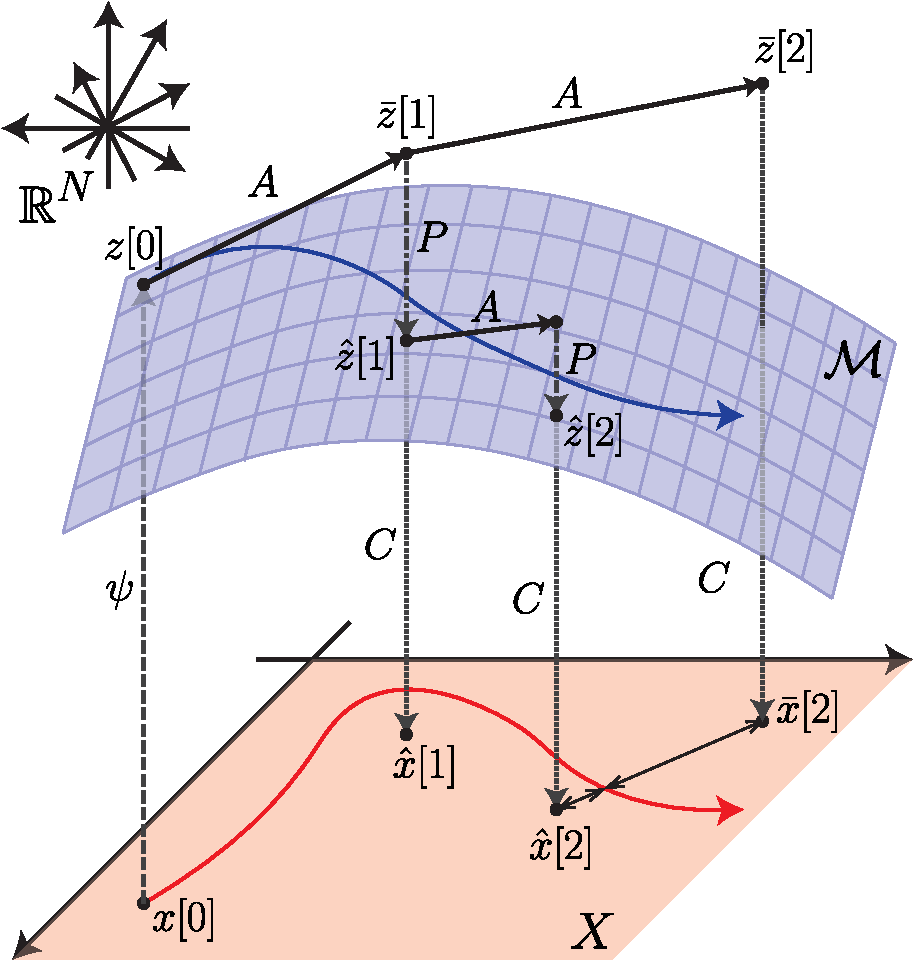
\includegraphics[width=0.9\linewidth]{figures/liftingManifold_v17.pdf}
    \caption{An illustration of the effect of deviating from the space image of the lifted functions ${\cal M}$ and how it can be remedied by defining a projection operation as described in Section \ref{subsec:sparsity}. 
    The evolution of the finite dimensional system in the state space $X$ from $x_0$ is depicted as a red curve. 
    The lifted version of this evolution is depicted as the blue curve which is a subset of the image of the lifting function.
    The discrete time system representation of the system in the infinite dimensional space created by iteratively defining $\bar{z}[j]= A\bar{z}[j]+Bu[j]$ may generate a solution that is outside of ${\cal M}$.
    Though one can still apply $C$ to $\bar{z}$ to project it back to $X$, this may result in poor performance.
    Instead by projecting $\bar{z}[j]$ onto the manifold at each discrete time step to define a new lifted state $\hat{z}[j]$ and defining further evolution from there, one can improve overall predictive performance. }
    \label{fig:manifold}
\end{figure}


%% Sysid algorithm
\begin{algorithm}[t]
\SetAlgoLined
\KwIn{ $\lambda$ , $\{ a[k] , b[k] \}$ and ${ u[k] }$ for $k = 1 , ... , K$}
\textbf{Step 1:} Lift data via \eqref{eq:lift} \\
\textbf{Step 2:} Combine lifted data and inputs via \eqref{eq:alpha} \\
\textbf{Step 3:} Approximate Koopman operator $\bar{U}_{T_s}$ via \eqref{eq:lasso} \\
\textbf{Step 4:} Extract model matrices $A,B$ via \eqref{eq:AB} \\
\textbf{Step 5:} Identify projection operator $P$ via \eqref{eq:P} \\
\KwOut{$\hat{A} := PA$, $\hat{B} := PB$   }
 \caption{Koopman Linear System Identification}
 \label{alg:mpc}
\end{algorithm}